% Trabajo sobre el modelo del hiperboloide
% Autores:
% * Margarita Gómez
% * Eva María González
% * David Melero
% * Mario Román
%
% Usando la plantilla de beamer de Pablo Baeyens.
% Autor: Pablo Baeyens (@pbaeyens)
% Email: pbaeyens31+github@gmail.com
% Licencia: CC BY-SA 3.0

%% Paquetes y configuración %

% Beamer
\PassOptionsToPackage{unicode}{hyperref}  % Evita errores con caracteres no ASCII
\PassOptionsToPackage{naturalnames}{hyperref} % tex.stackexchange.com/questions/10555
\documentclass[compress]{beamer}

% Idioma
\usepackage[spanish]{babel} % Traducciones
\usepackage[utf8]{inputenc} % Uso de caracteres UTF-8
\usepackage{lmodern}        % Fuentes de tamaño arbitrario
\usepackage[T1]{fontenc}    % Permite copiar y evita errores
\uselanguage{Spanish}       % Traducciones beamer
\languagepath{Spanish}      % (tex.stackexchange.com/questions/168208)

% Matemáticas
\usepackage{amsfonts}
\usepackage{amsmath}
\usepackage{amssymb}
\newtheorem*{axiom}{Axioma}

% Colores
\definecolor{backg}{HTML}{F2F2F2}    % Fondo
\definecolor{title}{HTML}{bdc3d1}    % Títulos
\definecolor{comments}{HTML}{BDBDBD} % Comentarios
\definecolor{keywords}{HTML}{08388c} % Palabras clave
\definecolor{strings}{HTML}{FA5858}  % Strings
\definecolor{links}{HTML}{2C2C95}    % Enlaces
\definecolor{bars}{HTML}{045FB4}     % Barras (gráfico)

% Código
\usepackage{listings}
\lstset{
language=[LaTeX]TeX,
basicstyle=\footnotesize,
morekeywords={href,uselanguage,languagepath,column},
otherkeywords={pause,usetheme,usecolortheme,useinnertheme,titlepage,tableofcontents,subtitle},
breaklines=true,
backgroundcolor=\color{backg},
keywordstyle=\color{keywords},
commentstyle=\color{comments},
stringstyle=\color{strings},
tabsize=2,
% Acentos, ñ, ¿, ¡ (tex.stackexchange.com/questions/24528)
extendedchars=true,
literate={á}{{\'a}}1 {é}{{\'e}}1 {í}{{\'i}}1 {ó}{{\'o}}1
         {ú}{{\'u}}1 {ñ}{{\~n}}1 {¡}{{\textexclamdown}}1
         {¿}{{?`}}1
}

% Gráficos
\usepackage{pgfplots}
\pgfplotsset{width=7cm,compat=1.8} % Opciones para gráficos

% Emoticonos
\usepackage{wasysym}

% tikz
\usepackage{tikz}
\usetikzlibrary{mindmap,trees,shadows}
\tikzset{ % Genera overlays
    invisible/.style={opacity=0},
    visible on/.style={alt={#1{}{invisible}}},
    alt/.code args={<#1>#2#3}{\alt<#1>{\pgfkeysalso{#2}}{\pgfkeysalso{#3}}},
}

%% Comandos %%
\newcommand{\ejemplo}[1]{\lstinputlisting{./examples/#1}} % Mostrar código de ejemplos
\newcommand{\muestra}[1]{\input{./examples/#1}}           % Mostrar ejemplos
\newcommand{\seccion}[1]{\input{./sections/#1}}           % Incluir secciones
\newcommand{\espacio}{\vspace*{\baselineskip}}            % Añade espacios
\newcommand{\beamer}{\texttt{beamer} }                    % Estilo único para beamer
\newcommand{\enlace}[3]{\href{#1}{\textbf{#2}} - {\small #3}}  % Estílo único para refs
\newcommand{\comando}[1]{{\color{black}\textbackslash}{\color{keywords}#1}}

\newcommand{\abs}[1]{\ensuremath\left\vert #1 \right\vert}
\newcommand{\norm}[1]{\ensuremath\left\Vert #1 \right\Vert}
\newcommand{\normt}[1]{\ensuremath\left\vert\kern-0.25ex\left\vert\kern-0.25ex\left\vert #1 \right\vert\kern-0.25ex\right\vert\kern-0.25ex\right\vert}

%% Temas %%
% Tema y tema de color
  \usetheme{Dresden}
  \usecolortheme{dolphin}
  \useinnertheme{circles}
  \setbeamercovered{transparent}
% Colores bloques
  \setbeamercolor{block title}{bg=title,fg=links}
  \setbeamercolor{block body}{bg=backg,fg=black}
  \setbeamercolor{block title alerted}{fg=red!70!black,bg=title!92!red}
  \setbeamercolor{block body alerted}{fg=black,bg=backg}
  \setbeamercolor{block title example}{fg=green!70!black,bg=title!92!green}
  \setbeamercolor{block body example}{fg=black,bg=backg}
% Enlaces (tex.stackexchange.com/questions/13423)
\hypersetup{colorlinks,linkcolor=,urlcolor=links}
% Quita enlaces de navegación (stackoverflow.com/questions/3017030)
\setbeamertemplate{navigation symbols}{}
% Quita barra inferior (stackoverflow.com/questions/1435837)
\setbeamertemplate{footline}{}
% Evita warnings boxes
\hfuzz=20pt
\vfuzz=20pt
% Evita wranings itemize
\renewcommand\textbullet{\ensuremath{\bullet}}

%% Título y otros %%
\title{Geometría hiperbólica}                                               % Título
\subtitle{Y otros modelos para la geometría hiperbólica}                                  % Subtítulo
\author[UGR]{ %
Eva Mª González \and Margarita Gómez  \\ David Melero \and Mario Román \texorpdfstring{\\
\href{}{}}{}} % Autor y e-mail
\date{Taller de geometría y topología}                                                            % Fecha


%% Presentación %%
\begin{document}

\begin{frame}
\titlepage
\end{frame}

\begin{frame}{Índice}
  \hypertarget{index}{}
  \tableofcontents
\end{frame}

\section{Introducción e historia}
\begin{frame}{Geometría hiperbólica}
  La \textbf{geometría hiperbólica} es el modelo axiomático que se
  obtiene al aceptar los cuatro primeros postulados de la geometría
  euclídea y sustituir el quinto postulado por el postulado de
  Lobachevsky. A pesar de este cambio, algunos aspectos y teoremas
  de la geometría euclídea que sean independientes del quinto postulado
  seguirán siendo válidos.
  
  \pause
  
  \begin{axiom}[Axioma de Lobachevsky]
    Dada una recta R y un punto P fuera de R, en el plano conteniendo a
    la línea R y al punto P existen al menos dos líneas distintas que pasan
    por P y no intersecan a R.
  \end{axiom}
\end{frame}

\begin{frame}{Historia}
  Históricamente, se han realizado esfuerzos por deducir el quinto
  postulado de Euclides de los otros cuatro.

  \begin{itemize}
  \item\textit{Giovanni Gerolamo Saccheri} intentó, en el siglo XVIII
    probarlo por reducción al absurdo y creó en el proceso un modelo
    incipiente de geometría hiperbólica que nunca llegó a formalizar
    en su creencia de que sería inconsistente.
  \item\textit{Johann Heinrich Lambert} estudió lo que constituirían
    los triángulos de la geometría hiperbólica probando que sus
    ángulos sumaban siempre menos que 180º. De hecho, probó que
    \[
      \pi - \alpha- \beta - \gamma = \mathrm{área}(T)k.
    \]
    Para $k$ una constante dependiente de la curvatura.
  \end{itemize}
\end{frame}

\begin{frame}{Historia}
  \begin{itemize}
  \item \textit{Carl Friedrich Gauss} trabajaría en un modelo similar
    sin publicar resultados.
    \pause
    
  \item La geometría hiperbólica que conocemos hoy surge en los años
    1820 gracias al trabajo independiente de \textit{János Bolyai} y
    \textit{Nikolai Ivanovich Lobachevsky}, que publicaron modelos que
    posibilitaban una geometría completamente consistente y sin el
    quinto postulado.
    \pause
    
  \item En 1968 \textit{Eugenio Beltrami} publicaría dos modelos del
    espacio hiperbólico que se hicieron conocidos por el uso que les
    darían \textit{Felix Klein} y \textit{Henri Poincaré}.
  \end{itemize}
\end{frame}
  
\section{Modelos de la geometría hiperbólica}
\begin{frame}{Modelo para un sistema}
  Un \textbf{modelo} para un sistema de postulados se define
  sustituyendo objetos específicos por los términos indefinidos del
  sistema que los cumplen.
  \pause
  
  \begin{exampleblock}{Ejemplo: geometría euclídea}
    Un modelo de la geometría euclídea es el que asigna a cada punto un par de reales $(a,b)$
    y a cada recta el conjunto de puntos que satisfacen una ecuación lineal $as+bt+u = 0$ para
    algunos reales tales que al menos uno de ellos no sea $0$.
  \end{exampleblock}
\end{frame}

\begin{frame}{Modelos de la geometría hiperbólica}
  Existen varios modelos de geometría hiperbólica:

  \begin{itemize}
  \item la \textbf{representación de Klein}, también conocida como el
    \textit{modelo proyectivo del disco} o \textit{modelo de
      Beltrami-Klein}, toma como puntos a los puntos interiores de
    un círculo en el plano euclídeo y como rectas a las cuerdaas del
    círculo.
    \pause
  
  \item el \textbf{modelo del disco de Poincaré}, usa también el
    interior de un círculo plano unidad como espacio de puntos,
    pero toma como rectas los arcos de circunferencia que cortan el
    borde del círculo plano de forma ortogonal.
    \pause
  
  \item el \textbf{modelo del hiperboloide} o \textit{de Lorentz} usa
    como espacio de puntos una hoja de un hiperboloide de dos hojas
    y como rectas los cortes de este con los hiperplanos del espacio
    de Minkowski en el que se embebe el hiperboloide.
  \end{itemize}
\end{frame}

\subsection{Modelo del hiperboloide}
\begin{frame}{Forma de Lorentz}
  El \textbf{modelo del hiperboloide} de la geometría hiperbólica se
  basa en la forma cuadrática de Lorentz,
  \[L(x,y,z)=x^2+y^2-z^2.\]

  Si pensamos en esta forma cuadrática como una norma, tendremos vectores
  distintos de cero con norma cero e incluso norma negativa. Esto nos da
  una clasificación de los vectores en

  \begin{enumerate}
  \item vectores espaciales, $x\in\mathbb{R}^3$ tales que $L(x)>0$; \pause
  \item vectores temporales, $x\in\mathbb{R}^3$ tales que $L(x)<0$; y \pause
  \item vectores luminosos, $x\in\mathbb{R}^3$ tales que $L(x)=0$.
  \end{enumerate}
\end{frame}

\begin{frame}{Hiperboloide}
  Con esta norma definimos
  \[\mathbb{H}^2=\{(x,y,z)\in\mathbb{R}^3 \mid L(x,y,z)=-1,\; (x,y,z) \cdot (0,0,1) > 0 \};\]
  y como vemos, esta es la hoja superior de un hiperboloide de dos
  hojas. Sabemos que es una superficie y por tanto localmente
  homeomorfo a un plano, por lo que lo llamaremos \textit{plano
    hiperbólico}.

  \begin{figure}[ht!]
    \centering
    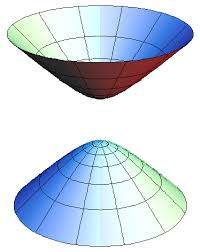
\includegraphics[width=0.2\textwidth]{hiperboloide.jpg}
  \end{figure}
\end{frame}

\begin{frame}{Modelo del hiperboloide}
  \begin{itemize}
  \item Los \textbf{puntos} en $\mathbb{H}$ serán los puntos de nuestro modelo
    de la geometría hiperbólica.
  \item Las \textbf{rectas} en el plano hiperbólico se definen como las intersecciones
    de $\mathbb{H}$ con planos que pasan por el origen. Las llamaremos
    \textit{rectas hiperbólicas}.
  \end{itemize}
  
  \begin{figure}[ht!]
    \centering
    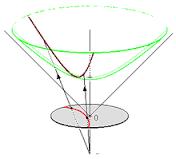
\includegraphics[width=0.4\textwidth]{hyperboloiddisc.png}
  \end{figure}
\end{frame}



\subsection{Disco de Poincaré}

\begin{frame}{Disco de Poincaré}
  El modelo de Poincaré se define tomando

  \begin{itemize}
  \item \textbf{puntos} como puntos contenidos en un círculo unidad. Es decir,
    como pares de reales $(a,b)$ cumpliendo $a^2+b^2 < 1$.
    \pause
  \item \textbf{líneas} como los puntos interiores al círculo unidad de otra circunferencia
    que lo corta perpendicularmente. Pueden definirse por ecuaciones de la forma
    \[x^2+y^2+ax+by+1=0.\]
    \pause
  \item los \textbf{ángulos} entre dos rectas hiperbólicas como el ángulo que
    proporcionan las tangentes a las rectas en el punto de corte.
  \end{itemize}
\end{frame}

\begin{frame}{Métrica en el disco de Poincaré}
  Si $u,v$ son dos vectores del espacio euclídeo $\mathbb{R}^n$,ambos
  con norma inferior a $1$, podemos definir un invariante isométrico de
  la siguiente manera:
  \[\delta (u,v)=2\frac{\norm{u-v}^2}{(1-\norm{u}^2)(1-\norm{v}^2)},\]

  donde $\norm{.}$ representa la norma euclídea usual. Definimos la
  función distancia como:
  \[d(u,v)=arccosh(1+\delta(u,v)).\]
\end{frame}

\begin{frame}{Métrica en el disco de Poincaré}
  Por ejemplo, en la siguiente imagen todos los puntos están a la misma
  distancia del punto $A$:

  \begin{figure}[ht!]
    \centering
    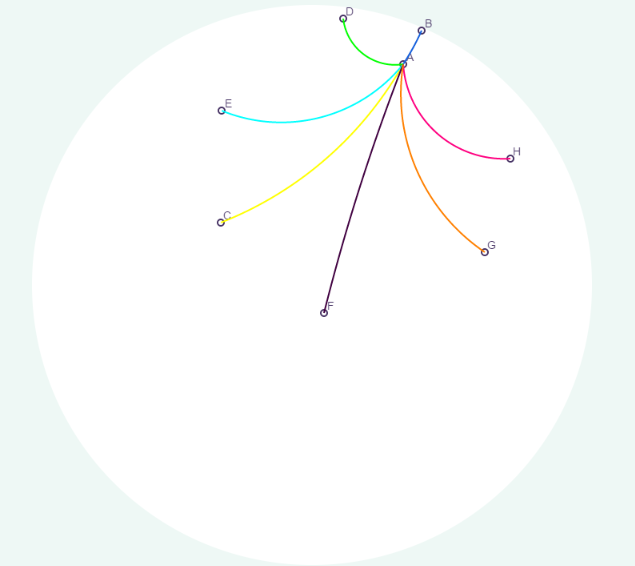
\includegraphics[width=0.7\textwidth]{Distancias.png}
  \end{figure}
\end{frame}

\begin{frame}{Recta por dos puntos}
  Dados dos puntos $u$ y $v$ en el disco que no estén en un diámetro, se
  puede resolver para el círculo de esta forma pasando por ambos puntos,
  y obtener
  \[\begin{aligned}
      x^{2}+y^{2} &+{\frac
        {u_{2}(v_{1}^{2}+v_{2}^{2})-v_{2}(u_{1}^{2}+u_{2}^{2})+u_{2}-v_{2}}{u_{1}v_{2}-u_{2}v_{1}}}x\\
      &+{\frac
      {v_{1}(u_{1}^{2}+u_{2}^{2})-u_{1}(v_{1}^{2}+v_{2}^{2})+v_{1}-u_{1}}{u_{1}v_{2}-u_{2}v_{1}}}y+1=0.
    \end{aligned}
  \]
\end{frame}

\begin{frame}{Relación con el modelo del hiperboloide}
  Los puntos del disco de Poincaré están en correspondencia con los puntos del modelo
  del hiperboloide. La correspondencia se obtiene proyectando desde el punto $(0,0,-1)$.

  \begin{itemize}
  \item Dado un punto $(x,y,z)$ en el hiperboloide (cumpliendo por tanto $z^2-x^2-y^2 = 1$),
    su proyección será
    \[\frac{1}{1+z}(x,y).\]
    \pause
  \item Dado un punto $(0,a,b)$ en el disco (cumpliendo por tanto $a^2+b^2 < 1$), su
    proyección será
    \[\frac{1}{1-a^2-b^2}\left(1+a^2+b^2,2a,2b\right).\]
  \end{itemize}
\end{frame}


\subsection{Disco de Beltrami-Klein}

\begin{frame}{Disco de Beltrami-Klein}
  El \textbf{modelo de Beltrami-Klein} interpreta como puntos los puntos
  del interior de un disco unidad y como líneas las cuerdas del círculo
  abiertas, en el sentido de que no se consideran en ella los puntos de
  la frontera del círculo.

  \begin{figure}[ht!]
    \centering
    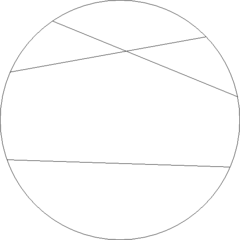
\includegraphics[width=0.4\textwidth]{beltramiklein.png}
  \end{figure}
\end{frame}

\begin{frame}{Métricas de Cayley-Kelvin}
  \begin{definition}
    Fijada una cuádrica $Q$ definimos la \textbf{distancia de Cayley-Kelvin}
    entre dos puntos como el logaritmo de una razón doble

    \[
      \mathrm{dist}(p,q) = C\log\frac{|qa||bp|}{|pa||bq|},
    \]

    donde $a$ y $b$ son los puntos en los que la recta que pasa por $p$
    y $q$ corta a $Q$. La $C$ es una constante arbitraria.
  \end{definition}
\end{frame}
  
\begin{frame}
  La métrica que usamos en nuestro caso en el disco de Klein es
  un caso particular de una métrica de Cayley-Kelvin cuando la cuádrica
  es el círculo:

  \[
    \mathrm{dist}(p,q) = \frac{1}{2}\log\frac{|qa||bp|}{|pa||bq|},
  \]

  donde $a,b$ son los puntos en los que la recta entre $p$ y $q$ corta
  al borde del disco unidad.

  \begin{theorem}
    Si desde el origen hasta un punto hay una distancia euclídea de $r$
    en la bola, la distancia hiperbólica entre ambos es
    \[
      \mathrm{dist}(o,p) = \frac{1}{2} \log\left(\frac{1+r}{1-r}\right) = \mathrm{artanh}(r),
    \]
    donde $\mathrm{artanh}$ es el arcotangente hiperbólico.
  \end{theorem}
\end{frame}

\begin{frame}{Distancias en el disco de Klein}
  \begin{figure}[ht!]
  \centering
  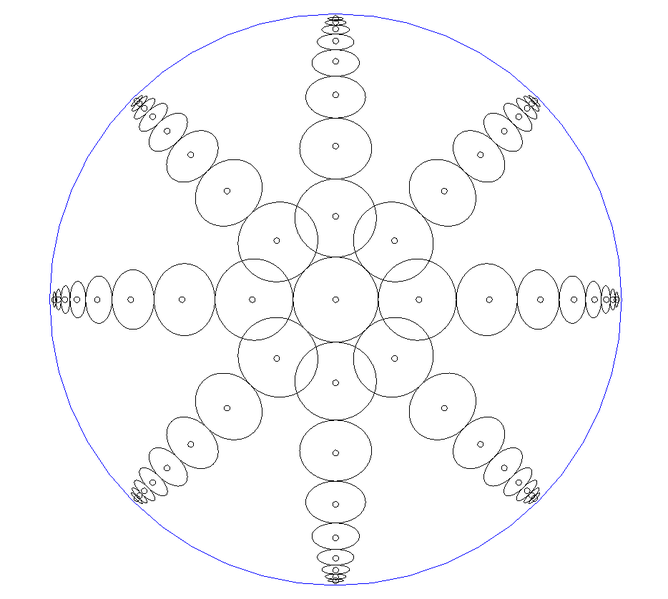
\includegraphics[width=60mm]{./kleinmodelcircles.png}
  \caption{Círculos en el disco de Klein. \textit{Wikimedia Commons}\label{kleincircles}}
\end{figure}
\end{frame}

\begin{frame}{Comparación con Poincaré}
  El modelo del disco de Klein preserva las líneas rectas como segmentos
  de recta dentro del disco, pero no es conforme; el disco de Poincaré,
  por otro lado, sí preserva los ángulos y es conforme, pero, como ya se
  ha mencionado, las rectas se convierten en segmentos de circunferencias
  ortogonales al disco.

  \begin{figure}[ht!]
    \centering
    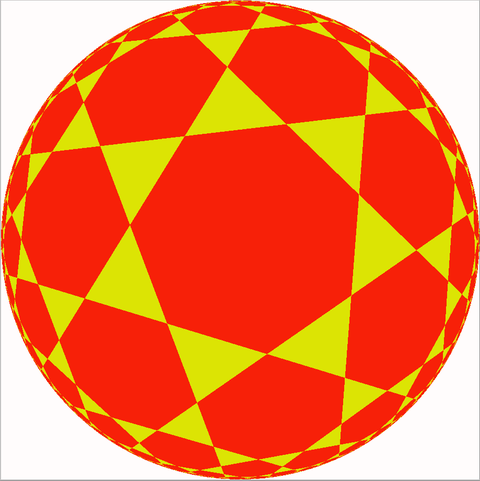
\includegraphics[width=30mm]{./klein37.png}
    \quad
    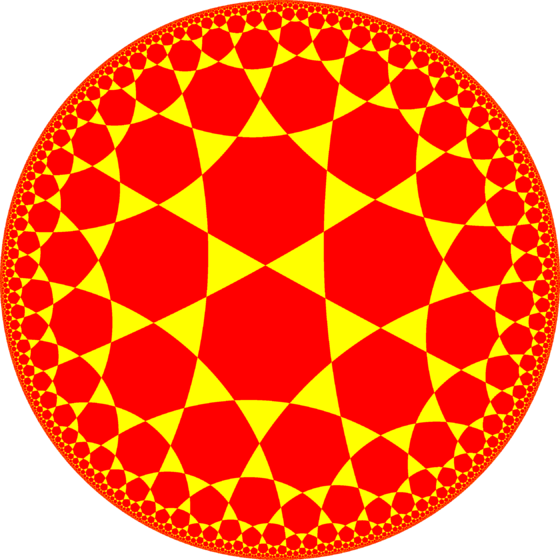
\includegraphics[width=30mm]{./poincare37.png}
    \caption{Comparación Klein-Poincaré. \textit{Wikimedia Commons} \label{kleinpoincare}}
  \end{figure}
\end{frame}


\section{Construcciones en el espacio hiperbólico}
\subsection{Cuadriláteros de Saccheri}
\begin{frame}{Cuadriláteros de Saccheri}
  \begin{definition}
    Un \textbf{cuadrilátero de Saccheri} es un cuadrilátero $ABCD$ con
    dos ángulos rectos adyacentes en $A$ y $B$ y con dos lados iguales
    $\overline{AD} = \overline{BC}$.
  \end{definition}
  \pause

  \begin{theorem}
    En un cuadrilátero de Saccheri, los dos ángulos no rectos son
    iguales.
  \end{theorem}

  \begin{figure}[ht!]
    \centering
    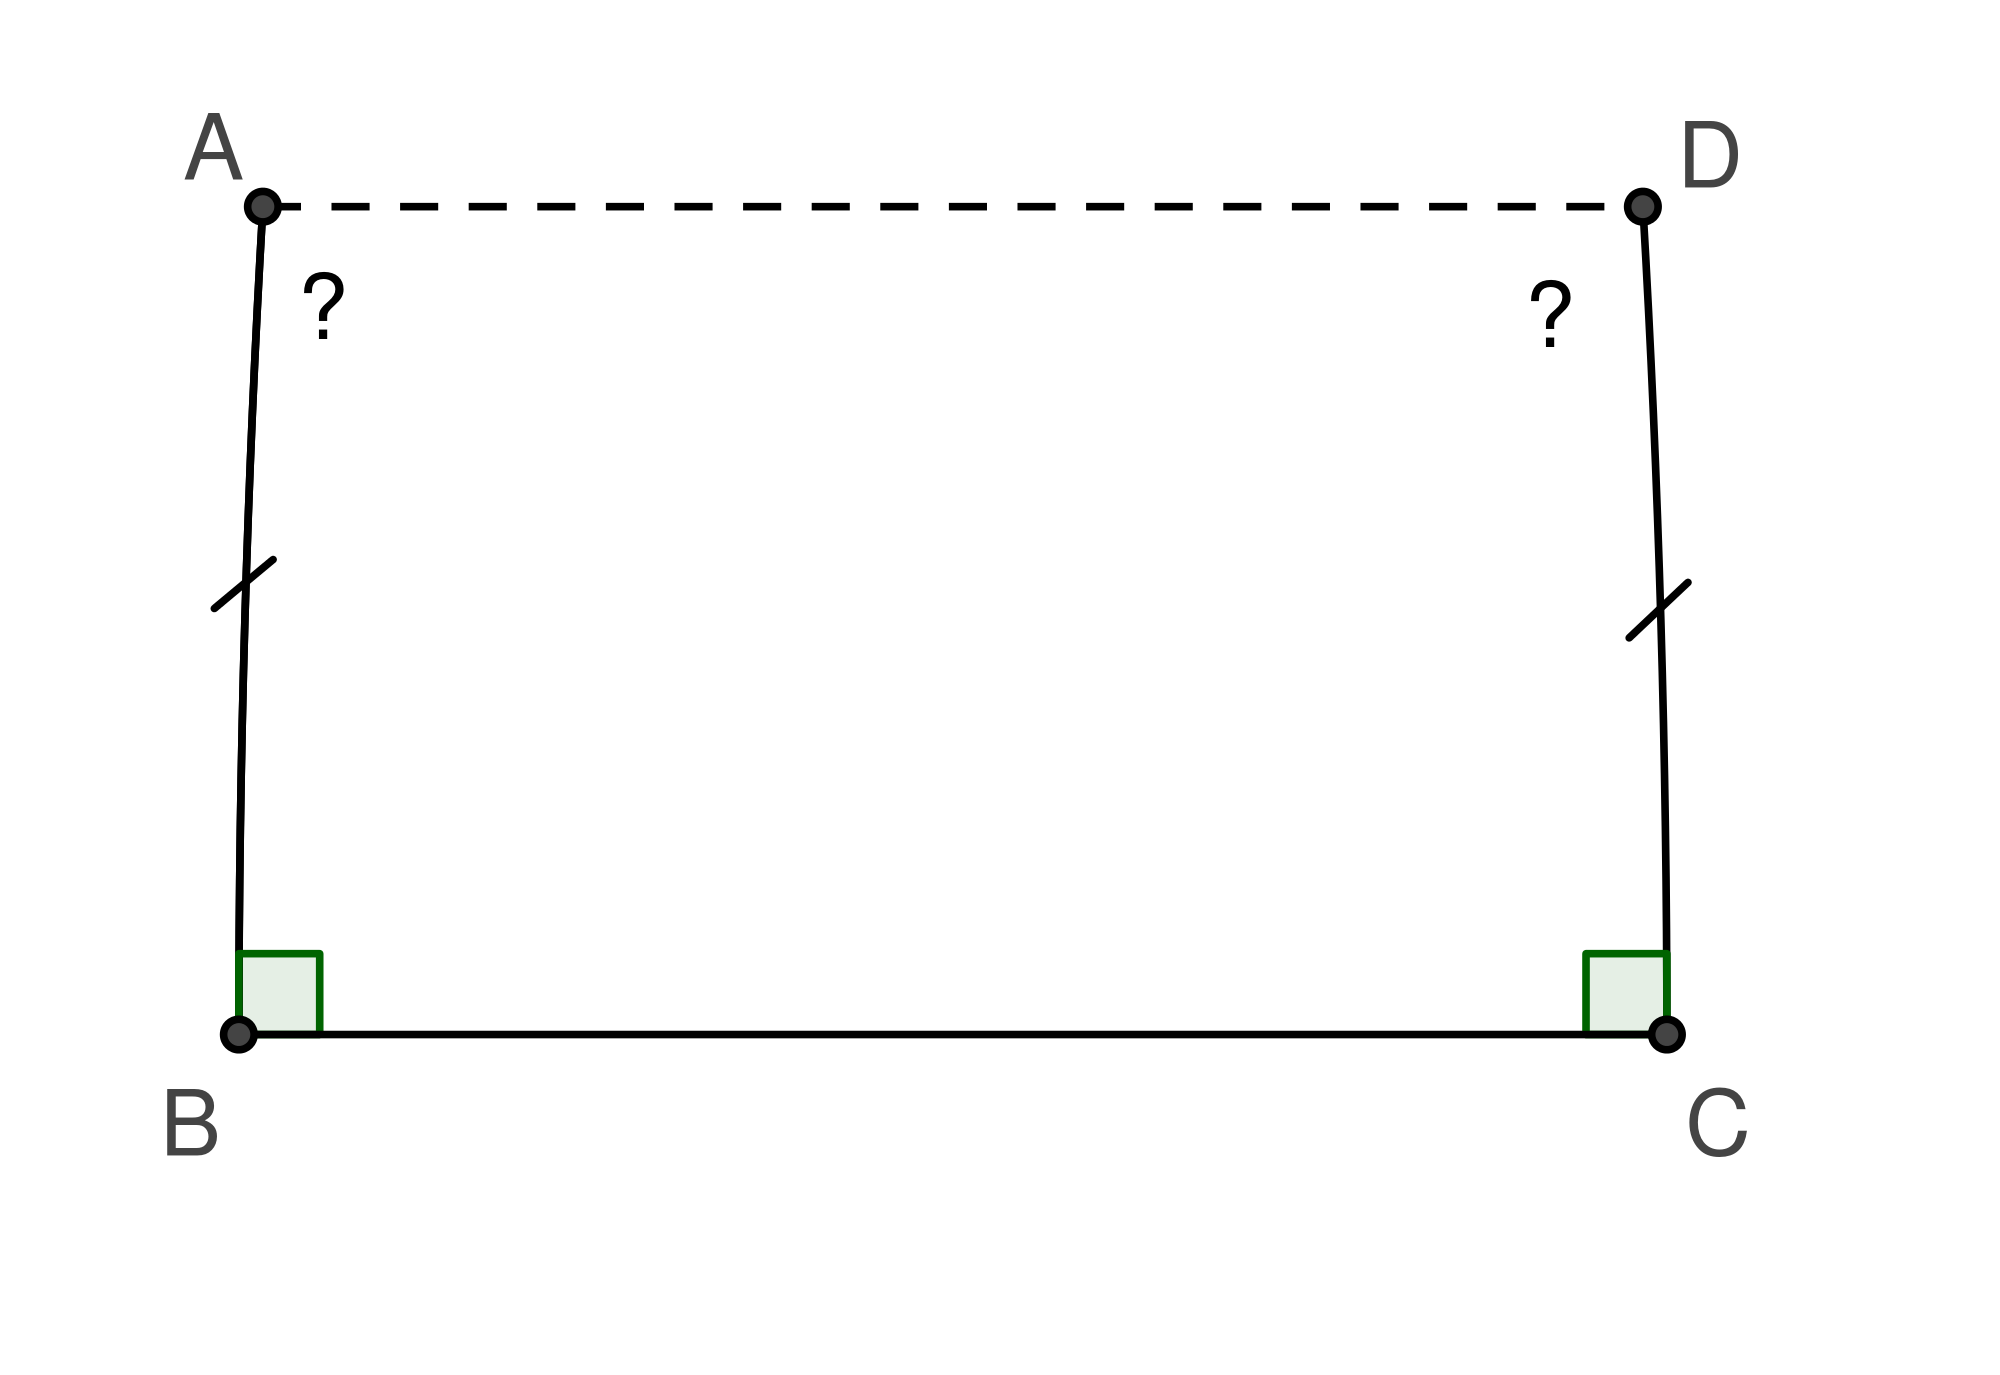
\includegraphics[width=30mm]{./saccheri.png}
    \caption{Cuadrilátero de Saccheri. \textit{Wikimedia Commons} \label{saccheri}}
  \end{figure}
\end{frame}


\subsection{Círculos, horociclos e hiperciclos}
\begin{frame}{Haces de rectas}
  Sabemos ya que dos rectas distintas en el espacio hiperbólico
  deben ser secantes, paralelas o ultraparalelas. Deberán por tanto
  pertenecer a uno de los siguientes conjuntos

  \begin{itemize}
  \item un \textbf{haz} de todas las rectas que pasan por un punto.
  \item un \textbf{haz de paralelas} con todas las rectas paralelas a un
    rayo dado.
  \item un \textbf{haz de ultraparalelas} con todas las líneas
    perpendiculares a una línea dada.
  \end{itemize}
\end{frame}

\begin{frame}{Círculos, horociclos e hiperciclos}
  \begin{definition}[Círculo]
    Dado un punto $C$ y un radio $r \geq 0$, llamamos \textbf{círculo}
    al conjunto de puntos a distancia $r$ de él, es decir,
    \[{\cal C} = \left\{ X \mid \mathrm{dist}(X,C) = r \right\}.\]
  \end{definition}

  \begin{definition}[Horociclo]
    Dado un haz de rectas paralelas a un rayo, definimos un \textbf{horociclo} como
    la órbita de un punto $C$ bajo las reflexiones determinadas por las rectas del
    haz. \cite{coxeter}
  \end{definition}

  \begin{definition}[Hiperciclo]
    Llamamos \textbf{hiperciclo} al lugar geométrico dado por los puntos a
    una distancia fija de una recta.
  \end{definition}
\end{frame}


\subsection{Polígonos}
\begin{frame}{Polígonos constructibles}
  \begin{theorem}
    Los ángulos constructibles en el plano euclídeo son exactamente los ángulos
    constructibles en el plano hiperbólico. \cite{jagy95}
  \end{theorem}
  
  Así, los polígonos regulares constructibles en el plano euclídeo serán
  constructibles en el plano hiperbólico. Simplemente es necesario
  formar el ángulo sobre una circunferencia y calcular los puntos de corte.
\end{frame}

\begin{frame}{Hexágono regular}
\end{frame}


\section{Referencias}
\begin{frame}{Bibliografía}
\begin{thebibliography}{9}

\bibitem{cedelberg89}
  Judith N. Cedelberg (1989-2001),
  A Course in Modern Geometries,
  New York: Springer Science and Business Media.

\bibitem{singer98}
  David A. Singer (1998),
  Geometry: Plane and Fancy,
  New York: Springer Science and Business Media.

\bibitem{ryan}
  Patrick J. Ryan
  Euclidean and non euclidean geometry. An analytic approach.

\bibitem{coxeter}
  Wiley; Coxeter,
  Introduction to Geometry.

\bibitem{jagy95}
  William Jagy (1995),
  Squaring Circles in the Hyperbolic Plane,
  The Mathematical Intelligencer.
  
\end{thebibliography}
\end{frame}
\end{document}
